%
% Copyright 2018 Joel Feldman, Andrew Rechnitzer and Elyse Yeager.
% This work is licensed under a Creative Commons Attribution-NonCommercial-ShareAlike 4.0 International License.
% https://creativecommons.org/licenses/by-nc-sa/4.0/
%
\questionheader{ex:s1.4}

\noindent
Recall that we are using $\log x$ to denote the logarithm of $x$ with
base $e$. In other courses it is often denoted $\ln x$.


%%%%%%%%%%%%%%%%%%
\subsection*{\Conceptual}
%%%%%%%%%%%%%%%%%%
\begin{Mquestion}\label{1.4_intbounds}
\begin{enumerate}[(a)]
\item True or False: $\displaystyle\int \sin(e^x)\cdot e^x\ \dee{x} = \left.\displaystyle\int \sin(u)\ \dee u\right|_{u=e^x} = -\cos(e^x)+C$
\item True or False: $\displaystyle\int_0^1 \sin(e^x)\cdot e^x\ \dee{x} = \displaystyle\int_0^1 \sin(u)\ \dee u = 1-\cos(1)$
\end{enumerate}
\end{Mquestion}
\begin{hint}
One is true, the other false.
\end{hint}
\begin{answer}
(a) true \qquad (b) false
\end{answer}
\begin{solution}
(a) This is true: it is an application of Theorem~\eref{CLP101}{thm subs
indef} in the CLP-2 text with $f(x)=\sin x$ and $u(x)=e^x$.

(b) This is false: the upper limit of integration is incorrect. Using
Theorem~\eref{CLP101}{thm subs def} in the CLP-2 text, the correct form
is \[\displaystyle\int_0^1 \sin(e^x)\cdot e^x\ \dee{x} = \displaystyle\int_1^{e} \sin(u)\ \dee u = -\cos(e) + \cos(1)
= \cos(1)-\cos(e).\]

Alternately, we can use the Fundamental Theorem of Calculus Part 2, and our answer from (a):
\[\int_0^1 \sin(e^x)\cdot e^x\ \dee{x}=\left[-\cos(e^x)+C\right]_{0}^1 = \cos(1)-\cos(e)\ .\]
\end{solution}


\begin{Mquestion}
Is the following reasoning sound? If not, fix it.
\begin{quote}
\emph{Problem:} Evaluate $\displaystyle\int (2x+1)^2 \dee{x}$.\\[10pt]
\emph{Work:} We use the substitution $u=2x+1$. Then:
\begin{align*}
\int (2x+1)^2 \dee{x}&=\int u^2\ \dee{u}\\
&=\frac{1}{3}u^3+C\\
&=\frac{1}{3}\left(2x+1\right)^3+C
\end{align*}

\end{quote}
\end{Mquestion}
\begin{hint}
You can check whether the final answer is correct by differentiating.
\end{hint}
\begin{answer}
The reasoning is not sound: when we do a substitution, we need to take care of the differential ($\dee{x}$). Remember the method of substitution comes from the chain rule: there should be a function \emph{and its derivative}. Here's the way to do it:
\begin{quote}
\emph{Problem:} Evaluate $\displaystyle\int (2x+1)^2 \dee{x}$.\\[10pt]
\emph{Work:} We use the substitution $u=2x+1$. Then $\dee{u}=2\dee{x}$, so $\dee{x} = \frac{1}{2}\dee{u}$:
\begin{align*}
\int (2x+1)^2 \dee{x}&=\int u^2\cdot \frac{1}{2}\ \dee{u}\\
&=\frac{1}{6}u^3+C\\
&=\frac{1}{6}\left(2x+1\right)^3+C
\end{align*}
\end{quote}

\end{answer}
\begin{solution}
The reasoning is not sound: when we do a substitution, we need to take care of the differential ($\dee{x}$). Remember the method of substitution comes from the chain rule: there should be a function \emph{and its derivative}. Here's the way to do it:
\begin{quote}
\emph{Problem:} Evaluate $\displaystyle\int (2x+1)^2 \dee{x}$.\\[10pt]
\emph{Work:} We use the substitution $u=2x+1$. Then $\dee{u}=2\dee{x}$, so $\dee{x} = \frac{1}{2}\dee{u}$:
\begin{align*}
\int (2x+1)^2 \dee{x}&=\int u^2\cdot \frac{1}{2}\ \dee{u}\\
&=\frac{1}{6}u^3+C\\
&=\frac{1}{6}\left(2x+1\right)^3+C
\end{align*}
\end{quote}

\end{solution}
%%%%%%%%%%%%%%%%%%%%

\begin{question}
Is the following reasoning sound? If not, fix it.
\begin{quote}
\emph{Problem:} Evaluate $\displaystyle\int_{1}^{\pi} \dfrac{\cos(\log t)}{t}\dee{t}$.\\[10pt]
\emph{Work:} We use the substitution $u=\log t$, so $\dee{u}=\frac{1}{t}\dee{t}$. Then:
\begin{align*}
\int_{1}^{\pi} \dfrac{\cos(\log t)}{t}\dee{t}&=\int_1^{\pi}\cos(u) \dee{u}\\
&=\sin(\pi)-\sin(1)=-\sin(1)\, .
\end{align*}
\end{quote}
\end{question}
\begin{hint}
Check the limits.
\end{hint}
\begin{answer}
The problem is with the limits of integration, as in Question~\ref{1.4_intbounds}. Here's how it ought to go:
\begin{quote}
\emph{Problem:} Evaluate $\displaystyle\int_{1}^{\pi} \dfrac{\cos(\log t)}{t}\dee{t}$.\\[10pt]
\emph{Work:} We use the substitution $u=\log t$, so $\dee{u}=\frac{1}{t}\dee{t}$. When $t=1$, we have $u=\log 1 =0$ and when $t=\pi$, we have $u=\log(\pi)$.
Then:
\begin{align*}
\int_{1}^{\pi} \dfrac{\cos(\log t)}{t}\dee{t}&=\int_{\log 1}^{\log(\pi)}\cos(u) \dee{u}\\
&=\int_{0}^{\log(\pi)}\cos(u) \dee{u}\\
&=\sin(\log(\pi))-\sin(0)=\sin(\log(\pi)) .
\end{align*}
\end{quote}
\end{answer}
\begin{solution}
The problem is with the limits of integration, as in Question~\ref{1.4_intbounds}. Here's how it ought to go:
\begin{quote}
\emph{Problem:} Evaluate $\displaystyle\int_{1}^{\pi} \dfrac{\cos(\log t)}{t}\dee{t}$.\\[10pt]
\emph{Work:} We use the substitution $u=\log t$, so $\dee{u}=\frac{1}{t}\dee{t}$.
When $t=1$, we have $u=\log 1 =0$ and when $t=\pi$, we have $u=\log(\pi)$. Then:
\begin{align*}
\int_{1}^{\pi} \dfrac{\cos(\log t)}{t}\dee{t}&=\int_{\log 1}^{\log(\pi)}\cos(u) \dee{u}\\
&=\int_{0}^{\log(\pi)}\cos(u) \dee{u}\\
&=\sin(\log(\pi))-\sin(0)=\sin(\log(\pi)) .
\end{align*}
\end{quote}

\end{solution}
%%%%%%%%%%%%%%%%%%%%

\begin{question}
Is the following reasoning sound? If not, fix it.
\begin{quote}
\emph{Problem:} Evaluate $\displaystyle\int_{0}^{\pi/4} x\tan (x^2) \ \dee{x}$.\\[10pt]
\emph{Work:} We begin with the substitution $u=x^2$,  $\dee{u} = 2x\dee{x}$:
\begin{align*}
\int_{0}^{\pi/4} x\tan (x^2) \ \dee{x}&= \int_{0}^{\pi/4} \frac{1}{2}\tan(x^2)\cdot 2x\dee{x}\\
&=\int_{0}^{\pi^2/16} \frac{1}{2}\tan u\ \dee{u}\\
&=\frac{1}{2}\int_{0}^{\pi^2/16} \dfrac{\sin u}{\cos u}\dee{u}
\intertext{Now we use the substitution $v=\cos u$, $\dee{v}=-\sin u \ \dee{u}$:}
&=\frac{1}{2}\int_{\cos 0}^{\cos(\pi^2/16)} -\dfrac{1}{v}\dee{v}\\
&=-\frac{1}{2}\int_{1}^{\cos(\pi^2/16)} \dfrac{1}{v}\dee{v}\\
&=-\frac{1}{2}\left[\log|v|\right]_{1}^{\cos(\pi^2/16)}\\
&=-\frac{1}{2}\left(\log\left(\cos(\pi^2/16)\right)-\log(1)\right)\\
&=-\frac{1}{2}\log\left(\cos(\pi^2/16)\right)
\end{align*}
\end{quote}
\end{question}
\begin{hint}
Check every step. Do they all make sense?
\end{hint}
\begin{answer}
This one is OK.
\end{answer}
\begin{solution}
Perhaps shorter ways exist, but the reasoning here is valid.

\begin{quote}
\emph{Problem:} Evaluate $\displaystyle\int_{0}^{\pi/4} x\tan (x^2) \ \dee{x}$.\\[10pt]
\emph{Work:} We begin with the substitution $u=x^2$,  $\dee{u} = 2x\dee{x}$: \\
\textcolor{red}{If $u=x^2$, then $\diff{u}{x} = 2x$, so indeed $\dee{u}=2x\dee{x}$.}
\begin{align*}
\int_{0}^{\pi/4} x\tan (x^2) \ \dee{x}&= \int_{0}^{\pi/4} \frac{1}{2}\tan(x^2)\cdot 2x\dee{x}&\color{red}\mbox{algebra}\\
&=\int_{0}^{\pi^2/16} \frac{1}{2}\tan u\ \dee{u}
\intertext{\color{red}\mbox{Every piece is changed from $x$ to $u$: integrand, differential, limits.}}
&=\frac{1}{2}\int_{0}^{\pi^2/16} \dfrac{\sin u}{\cos u}\dee{u}
&\color{red} \tan u = \frac{\sin u}{\cos u}\\
\intertext{Now we use the substitution $v=\cos u$, $\dee{v}=-\sin u \ \dee{u}$:}
&=\frac{1}{2}\int_{\cos 0}^{\cos(\pi^2/16)} -\dfrac{1}{v}\dee{v}
\intertext{\color{red}\mbox{Every piece is changed from $u$ to $v$: integrand, differential, limits.}}
&=-\frac{1}{2}\int_{1}^{\cos(\pi^2/16)} \dfrac{1}{v}\dee{v}&\color{red} \cos(0)=1\\
&=-\frac{1}{2}\bigg[\log|v|\bigg]_{1}^{\cos(\pi^2/16)}&\color{red}\mbox{FTC Part 2}\\
&=-\frac{1}{2}\left(\log\left(\cos(\pi^2/16)\right)-\log(1)\right)\\
&=-\frac{1}{2}\log\left(\cos(\pi^2/16)\right)&\color{red} \log(1)=0
\end{align*}
\end{quote}

\end{solution}
%%%%%%%%%%%%%%%%%%%%

\begin{Mquestion}[2016A]
What is the integral that results when the substitution $u= \sin x$   is applied
to the integral $\displaystyle \int_0^{\pi/2} f(\sin x)\,\dee{x}$?
\end{Mquestion}

%\begin{hint}
%\end{hint}

\begin{answer}
 $\displaystyle\int_{0}^{1} \frac{f(u)}{\sqrt{1-u^2}}\,\dee{u}$.
Because the denominator $\sqrt{1-u^2}$ vanishes when $u=1$, this is what is known as an improper integral. Improper integrals will be discussed in 
\S~\eref{CLP101}{sec improp int} of the CLP-2 text.
\end{answer}

\begin{solution}
We substitute:
\begin{align*}
u&=\sin x, \\
\dee{u}&=\cos x\,\dee{x}, \\
\cos x &= \sqrt{1-\sin^2 x}=\sqrt{1-u^2},\\
\dee{x} &=\dfrac{\dee{u}}{\cos x} = \dfrac{\dee{u}}{\sqrt{1-u^2}}\\
u(0)&=\sin 0 = 0\\
u\left(\frac{\pi}{2}\right)&=\sin\left(\frac{\pi}{2}\right)=1
\intertext{So,}
     \int_{x=0}^{x=\pi/2} f(\sin x)\,\dee{x}
&= \int_{u=0}^{u=1} f(u)\,\frac{\dee{u}}{\sqrt{1-u^2}}
\end{align*}
Because the denominator $\sqrt{1-u^2}$ vanishes when $u=1$, this is what is known as an improper integral. Improper integrals will be discussed in 
\S~\eref{CLP101}{sec improp int} of the CLP-2 text.
\end{solution}
%%%%%%%%%%%%%%%%%%%

\begin{question}
Let $f$ and $g$ be functions that are continuous and differentiable everywhere. Simplify \[\int f'(g(x))g'(x)\ \dee{x} - f(g(x)).\]
\end{question}
\begin{hint}
What is $\diff{}{x}\{f(g(x))\}$?
\end{hint}
\begin{answer}
some constant $C$
\end{answer}
\begin{solution}
Using the chain rule, we see that
\[\diff{}{x}\{f(g(x))\}=f'(g(x))g'(x)\]
So, $\textcolor{red}{f(g(x))}$ is an antiderivative of $\textcolor{red}{f'(g(x))g'(x)}$. All antiderivatives of $f'(g(x))g'(x)$ differ by only a constant, so:
\begin{align*}
\textcolor{red}{\int f'(g(x))g'(x)\ \dee{x}} - f(g(x))&=\textcolor{red}{f(g(x))+C}-f(g(x))\\
&=C
\end{align*}
That is, our expression simplifies to some constant $C$.

Remark: since
\[\int f'(g(x))g'(x)\ \dee{t} - f(g(x))=C\]
we conclude
\[\int f'(g(x))g'(x)\ \dee{t} = f(g(x))+C\]
which is precisely how we perform substitution on integrals.
\end{solution}
%%%%%%%%%%%%%%%%%%%



%%%%%%%%%%%%%%%%%%
\subsection*{\Procedural}
%%%%%%%%%%%%%%%%%%


\begin{question}[2016Q2]
Use substitution to evaluate $\displaystyle\int_{0}^{1} x e^{x^2} \cos (e^{x^2}) \,\dee{x}$.
\end{question}

\begin{hint}
What is the derivative of the argument of the cosine?
\end{hint}

\begin{answer}
$\dfrac{1}{2}\big( \sin(e) - \sin(1) \big)$
\end{answer}

\begin{solution}
We write $\textcolor{red}{u(x) = e^{x^2}}$ and find $\textcolor{blue}{\dee{u} = u'(x)\,\dee{x}=2x e^{x^2}\dee{x}}$. Note that $u(1)=e^{1^2}=e$ when $x=1$, and $u(0)=e^{0^2}=1$ when $x=0$. Therefore:
\begin{align*}
\int_{0}^{1} \textcolor{blue}{x e^{x^2}} \cos (\textcolor{red}{e^{x^2}}) \,\textcolor{blue}{\dee{x}} &= \textcolor{blue}{\frac{1}{2}}\int_{x=0}^{x=1} \cos (\textcolor{red}{u(x)}) \textcolor{blue}{u'(x)\,\dee{x} }\\
&=\textcolor{blue}{ \frac{1}{2}}\int_{u=1}^{u=e} \cos(\textcolor{red}u)\,\color{blue}\dee{u}\\
&= \frac{1}{2}\bigg[\sin(u) \bigg]_1^e
= \frac{1}{2}\big( \sin(e) - \sin(1) \big).
\end{align*}
\end{solution}
%%%%%%%%%%%%%%%%%%%

\begin{question}[2001D]
Let $f(t)$ be any function for which $\displaystyle\int_1^8 f(t)\,\dee{t}=1$.
Calculate the integral $\displaystyle\int_1^2 x^2 f(x^3)\,\dee{x}$.
\end{question}

\begin{hint}
What is the title of the current section?
\end{hint}

\begin{answer}
$\dfrac{1}{3}$
\end{answer}

\begin{solution}
Substituting $\textcolor{red}{y=x^3}$, $\textcolor{blue}{\dee{y}=3x^2\ \dee{x}}$\ :
\begin{align*}
\int_1^2 \textcolor{blue}{x^2} f(\textcolor{red}{x^3})\,\textcolor{blue}{\dee{x}}
=\textcolor{blue}{\frac{1}{3}}\int_1^8 f(\textcolor{red}{y})\,\textcolor{blue}{\dee{y}}
=\frac{1}{3}
\end{align*}
\end{solution}
%%%%%%%%%%%%%%%%%%%

\begin{Mquestion}[M121 2014A]
Evaluate $\displaystyle \int  \frac{x^2}{{(x^3+1)}^{101}}\dee{x}$.
\end{Mquestion}

\begin{hint}
What is the derivative of $x^3+1$?
\end{hint}

\begin{answer}
$-\dfrac{1}{300{(x^3+1)}^{100}} + C$
\end{answer}

\begin{solution}
Setting $\textcolor{red}{u=x^3+1}$, we have $\textcolor{blue}{\dee{u} = 3x^2\,\dee{x}}$ and so
\begin{align*}
 \int  \frac{\textcolor{blue}{x^2\,\dee{x}}}{{(\textcolor{red}{x^3+1})}^{101}}
  &= \int \frac{\textcolor{blue}{\dee{u}/3}}{\textcolor{red}{u}^{101}}\\
  &=\frac{1}{3}\int u^{-101}\ \dee{u}\\
&=\frac{1}{3}\cdot\dfrac{u^{-100}}{-100}\\
  &= -\frac{1}{3\times 100 u^{100}} + C\\
  &=-\frac{1}{300{(x^3+1)}^{100}} + C
\end{align*}
\end{solution}
%%%%%%%%%%%%%%%%%%%



\begin{Mquestion}[2016Q2]
Evaluate $\displaystyle \int_{e}^{e^4} \frac{\dee{x}}{x\log x}$.
\end{Mquestion}

\begin{hint}
What is the derivative of $\log x$?
\end{hint}

\begin{answer}
$\log 4$
\end{answer}

\begin{solution}
Setting $\textcolor{red}{u=\log x}$, we have $\textcolor{blue}{\dee{u} = \frac{1}{x}\,\dee{x}}$ and so
\begin{equation*}
 \int_{e}^{e^4} \frac{\textcolor{blue}{\dee{x}}}{\textcolor{blue}x\cdot\textcolor{red}{\log x}}
  = \int_{x=e}^{x=e^4} \frac1{\textcolor{red}{\log x}} \cdot \textcolor{blue}{\frac{1}{x}\,\dee{x} }
  = \int_{u=1}^{u=4} \frac{1}{\textcolor{red}u}\,\textcolor{blue}{ \dee{u}},
\end{equation*}
since $u=\log(e)=1$ when $x=e$ and $u=\log(e^4)=4$ when $x=e^4$.
Then, by the Fundamental Theorem of Calculus Part 2,
\begin{equation*}
\int_{1}^{4} \frac{1}{u}\, \dee{u}
   = \Big[\log |u| \Big]_{1}^{4} = \log 4 - \log 1 = \log 4.
\end{equation*}
\end{solution}
%%%%%%%%%%%%%%%%%%%

\begin{question}[2012A]
Evaluate $\displaystyle \int_{0}^{\pi/2} \frac{\cos x} {1+\sin x}\,\dee{x}$.
\end{question}

\begin{hint}
What is the derivative of $1+\sin x$?
\end{hint}

\begin{answer}
$\log 2 $
\end{answer}

\begin{solution}
Setting $\textcolor{red}{u=1+\sin x}$, we have $\textcolor{blue}{\dee{u} = \cos x~\dee{x}}$ and so
\begin{equation*}
 \int_{0}^{\pi/2} \frac{\textcolor{blue}{\cos x}} {\textcolor{red}{1+\sin x}} \textcolor{blue}{\dee{x} }
  = \int_{x=0}^{x=\pi/2} \frac{1}{\textcolor{red}{1+\sin x}}\, \textcolor{blue}{\cos x ~\dee{x} }
   = \int_{u=1}^{u=2} \frac{\textcolor{blue}{\dee{u}}}{\textcolor{red}u}
\end{equation*}
since $u=1+\sin 0=1$ when $x=0$ and $u=1+\sin(\pi/2)=2$ when $x=\pi/2$.
Then, by the Fundamental Theorem of Calculus Part 2,
\begin{equation*}
\int_{u=1}^{u=2} \frac{\dee{u}}{u}
  = \Big[\log|u| \Big]_{1}^{2} = \log 2
\end{equation*}
\end{solution}
%%%%%%%%%%%%%%%%%%%



\begin{question}[2016Q2]
Evaluate $\displaystyle \int_{0}^{\pi/2} \cos x \cdot (1+\sin^2 x)\,\dee{x}$.
\end{question}

\begin{hint}
$\cos x$ is the derivative of what?
\end{hint}

\begin{answer}
$\dfrac{4}{3}$
\end{answer}

\begin{solution}
Setting $\textcolor{red}{u=\sin x}$, we have $\textcolor{blue}{\dee{u} = \cos x~\dee{x}}$ and so
\begin{equation*}
 \int_{0}^{\pi/2} \textcolor{blue}{\cos x} \cdot (1+\textcolor{red}{\sin}^2 \textcolor{red}x)\textcolor{blue}{\dee{x} }
  = \int_{x=0}^{x=\pi/2} (1+\textcolor{red}{\sin}^2 \textcolor{red}{x})\cdot \textcolor{blue}{\cos x ~\dee{x} }
   = \int_{u=0}^{u=1} (1+\textcolor{red}{u}^2) \,\textcolor{blue}{\dee{u}},
\end{equation*}
since $u=\sin 0=0$ when $x=0$ and $u=\sin(\pi/2)=1$ when $x=\pi/2$. Then, by the Fundamental Theorem of Calculus Part 2,
\begin{equation*}
\int_{0}^{1} (1+u^2) \,\dee{u}
  = \left[u+\frac{u^3}{3} \right]_{0}^{1} =\left(1+\frac{1}{3}\right) -0 = \frac{4}{3}.
\end{equation*}
\end{solution}
%%%%%%%%%%%%%%%%%%%


\begin{question}[2013A]
Evaluate
$\displaystyle\int_1^3(2x-1)e^{x^2-x}\ \dee{x}$.
\end{question}

\begin{hint}
What is the derivative of the exponent?
\end{hint}

\begin{answer}
$e^6-1$
\end{answer}

\begin{solution}
Substituting $\textcolor{red}{t=x^2-x}$,  $\textcolor{blue}{\dee{t} = (2x-1)\,\dee{x}}$ and noting that $t=0$
when $x=1$ and $t=6$ when $x=3$,
\begin{align*}
\int_1^3 \textcolor{blue}{(2x-1)}e^{\textcolor{red}{x^2-x}}\textcolor{blue}{ \dee{x}}
&=  \int_0^6 e^{\textcolor{red}t}\ \textcolor{blue}{\dee{t} }
=\big[e^t\big]_0^6
=e^6-1
\end{align*}

\end{solution}
%%%%%%%%%%%%%%%%%%%


\begin{Mquestion}[2016Q2]
Evaluate ${\displaystyle \int \frac{(x^2-4)x}{\sqrt{4-x^2}}\,\dee{x}}$.
\end{Mquestion}

\begin{hint}
What is the derivative of the argument of the square root?
\end{hint}

\begin{answer}
$\dfrac{1}{3}(4-x^2)^{3/2}+C$
\end{answer}

\begin{solution}
We use the substitution $\textcolor{red}{u=4-x^2}$, for which $\textcolor{blue}{\dee{u}=-2x\,\dee{x}}$\,:
\begin{align*}
\int \frac{x^2-4}{\sqrt{4-x^2}}\,x\,\dee{x}
&=\int \frac{1}{2}\cdot\frac{\textcolor{red}{4-x^2}}{\sqrt{\textcolor{red}{4-x^2}}}\textcolor{blue}{ ({-}2x)\,\dee{x}} \\
&=\frac{1}{2} \int \frac{\textcolor{red}u}{\sqrt{\textcolor{red}u}}\,\textcolor{blue}{\dee{u} }\\
&=\frac{1}{2}\int \sqrt{u}\,\dee{u} \\
&=\frac{1}{2}\frac{u^{3/2}}{3/2}+C\\
&=\frac{1}{3}(4-x^2)^{3/2}+C
\end{align*}
\end{solution}
%%%%%%%%%%%%%%%%%%%

%%%%%%%%%%%%%%%%%%%
\begin{question}
Evaluate $\displaystyle\int \dfrac{e^{\sqrt{\log x}}}{2x\sqrt{\log x}}\ \dee{x}$\,.
\end{question}
\begin{hint}
What is $\diff{}{x}\left\{\sqrt{\log x}\right\}$?
\end{hint}
\begin{answer}
$e^{\sqrt{\log x}}+C$
\end{answer}
\begin{solution}
\begin{description}
\item[Solution 1:]
If we let $\textcolor{red}{u=\sqrt{\log x}}$, then $\textcolor{blue}{\dee{u}=\dfrac{1}{2x\sqrt{\log x}}\ \dee{x}}$, and:
\begin{align*}
\int \dfrac{e^{\textcolor{red}{\sqrt{\log x}}}}{\textcolor{blue}{2x\sqrt{\log x}}}\ \textcolor{blue}{\dee{x}}&=\int  e^{\textcolor{red}u}\ \textcolor{blue}{\dee{u}}=e^u+C=e^{\sqrt{\log x}}+C
\end{align*}
\item[Solution 2:] In Solution 1, we made a pretty slick choice. We might have tried to work with something a little less convenient. For example, it's not unnatural to think that $\textcolor{red}{u=\log x}$, $\textcolor{blue}{\dee{u}=\dfrac{1}{x}\ \dee{x}}$ would be a good choice. In that case:
\begin{align*}
\int \dfrac{e^{\sqrt{\textcolor{red}{\log x}}}}{2\textcolor{blue}{x}\sqrt{\textcolor{red}{\log x}}}\ \textcolor{blue}{\dee{x}}&=
\int \frac{e^{\sqrt{\textcolor{red}u}}}{2\sqrt{\textcolor{red}u}}\textcolor{blue}{\dee{u}}
\intertext{Now, we should be able to see that $\textcolor{orange}{w=\sqrt{u}}$, $\textcolor{purple}{\dee{w} = \dfrac{1}{2\sqrt{u}}\ \dee{u}}$ is a good choice:}
\int\frac{e^{\textcolor{orange}{\sqrt{u}}}}{\textcolor{purple}{2\sqrt{u}}}\
\textcolor{purple}{\dee{u}}
&=\int e^{\textcolor{orange}w}\ \textcolor{purple}{\dee{w}}\\
&=e^{\sqrt{u}}+C\\
&=e^{\sqrt{\log x}}+C
\end{align*}

\end{description}
\end{solution}





%%%%%%%%%%%%%%%%%%
\subsection*{\Application}
%%%%%%%%%%%%%%%%%%

\begin{question}[2016A]
Calculate $\displaystyle\int_{-2}^2 xe^{x^2}\,\dee{x}$.
\end{question}

\begin{hint}
There is a short, slightly sneaky method --- guess an antiderivative ---
and a really short, still-more-sneaky method.
\end{hint}

\begin{answer}
$0$
\end{answer}

\begin{solution}
\begin{description}
\item[The straightforward method:]
We use the substitution $\textcolor{red}{u=x^2}$, for which $\textcolor{blue}{\dee{u}=2x\,\dee{x}}$, and note that
$u=4$ for both $x=2$ and $x=-2$:
\begin{align*}
\int_{-2}^2 xe^{x^2}\,\dee{x}
=\int_{-2}^2 \frac{1}{2}e^{\textcolor{red}{x^2}}\,\textcolor{blue}{2x\dee{x}} 
= \int_4^4 \frac{1}{2}e^{\textcolor{red}{u}}\,\textcolor{blue}{\dee{u}}
=0
\end{align*}

\item[The slightly sneaky method:]
We note that $\displaystyle\diff{}{x} \left\{e^{x^2} \right\}= 2x\, e^{x^2}$, so that $\dfrac{1}{2} e^{x^2}$
is a antiderivative for the integrand $x e^{x^2}$. So
\begin{align*}
\int_{-2}^2 xe^{x^2}\,\dee{x} = \bigg[\frac{1}{2}e^{x^2}\bigg]_{-2}^2
=\frac{1}{2}e^4-\frac{1}{2}e^4=0
\end{align*}


\item[The really sneaky method:]
The integrand $f(x) = x e^{x^2}$ is an odd function (meaning that $f(-x)=-f(x)$).
So by Theorem \eref{CLP101}{thm:INTevenodd} in the  CLP-2 text every integral
of the form $\int_{-a}^a x e^{x^2}\,\dee{x}$ is zero.
\end{description}
\end{solution}
%%%%%%%%%%%%%%%%%%%



\begin{question}[2000D]
Calculate $\displaystyle\lim\limits_{n\rightarrow\infty}\sum\limits_{j=1}^n
\dfrac{j}{n^2}\sin\left(1+\dfrac{j^2}{n^2}\right)$.
\end{question}

\begin{hint}
Review the definition of the definite integral and in particular
Definitions  \eref{CLP101}{def:INTintegral}  and
                 \eref{CLP101}{def:INTthreeRiemannSums} in the
%\href{http://www.math.ubc.ca/%7Efeldman/m101/clp/clp_notes_101.pdf}{CLP 101 notes}.
CLP-2 text.
\end{hint}

\begin{answer}
$\dfrac{1}{2}[\cos 1-\cos 2]\approx0.478$
\end{answer}

\begin{solution}
The given sum is of the form
\begin{align*}
\lim_{n\rightarrow\infty}\sum_{j=1}^n
\frac{j}{n^2}\sin\Big(1+\frac{j^2}{n^2}\Big)
=\lim_{n\rightarrow\infty}\sum_{j=1}^n
f(x_j^*)\De x
\end{align*}
with $\De x=\frac{1}{n}$, $x_j^*=\frac{j}{n}$ and $f(x)=x\sin(1+x^2)$.
Since $x_0^*=0$ and $x_n^*=1$, the right hand side is the definition
(using the right Riemann sum) of
\begin{align*}
\int_0^1 f(x)\,\dee{x}
&=\int_0^1 x\sin(1+x^2)\,\dee{x} \\
&=\frac{1}{2}\int_1^2 \sin(y)\,\dee{y}\qquad\text{with $y=1+x^2$, $\dee{y}=2x\,\dee{x}$} \\
&=\frac{1}{2}\Big[-\cos(y)\Big]_{y=1}^{y=2} \\
&=\frac{1}{2}[\cos 1-\cos 2]
\end{align*}
Using a calculator, we see this is close to $0.478$.
\end{solution}
%%%%%%%%%%%%%%%%%%%

\Instructions{Questions~\ref{1.4_roughsuba} through \ref{1.4_roughsubb} can be solved by substitution, but it may not be obvious which substitution will work. In general, when evaluating integrals, it is not always immediately clear which methods are appropriate. If this happens to you, don't despair, and definitely don't give up! Just guess a method and try it. Even if it fails, you'll probably learn something that you can use to make a better guess.\footnote{This is also pretty decent life advice.}}

\begin{Mquestion}\label{1.4_roughsuba} Evaluate $\displaystyle\int_{0}^1 \dfrac{u^3}{u^2+1}\ \dee{u}$.
\end{Mquestion}
\begin{hint}
If $w=u^2+1$, then $u^2=w-1$.
\end{hint}
\begin{answer}
$\dfrac{1}{2}-\dfrac{1}{2}\log 2$
\end{answer}
\begin{solution}
Often, the denominator of a function is a good guess for the substitution. So, let's try setting $\textcolor{red}{w=u^2+1}$. Then $\textcolor{blue}{\dee{w}=2u\ \dee{u}}$:
\begin{align*}
\int_{0}^1 \dfrac{u^3}{u^2+1}\ \dee{u}&=
\frac{1}{2}\int_{0}^1 \dfrac{u^2}{\textcolor{red}{u^2+1}}\ \textcolor{blue}{2u\ \dee{u}}
\intertext{The numerator now is $u^2$, and looking at our substitution, we see $\textcolor{red}{u^2=w-1}$:}
&=\frac{1}{2}\int_{1}^2 \dfrac{\textcolor{red}{w-1}}{\textcolor{red}{w}}\ \textcolor{blue}{\dee{w}}\\
&=\frac{1}{2}\int_{1}^2 \left(1 - \frac{1}{w}\right)\dee{w}\\
&=\frac{1}{2}\left[w - \log|w|\right]_{w=1}^{w=2}\\
&=\frac{1}{2}\left(2-\log 2 - 1\right)=\frac{1}{2}-\frac{1}{2}\log 2
\end{align*}
\end{solution}

%%%%%%%%%%%%%%%%%%%

\begin{question} Evaluate $\displaystyle\int \tan^3 \theta\  \dee{\theta}$\ .
\end{question}
\begin{hint}
Using a trigonometric identity, this is similar (though not identical) to $\int \tan \theta \cdot \sec^2 \theta\ \dee{\theta}$.
\end{hint}
\begin{answer}
$\frac{1}{2}\tan^2\theta
-\log|\sec \theta|+C$
\end{answer}
\begin{solution}
The only thing we really have to work with is a tangent, so it's worth considering what would happen if we substituted
$\textcolor{red}{u=\tan \theta}$.
Then $\textcolor{blue}{\dee{u}=\sec^2\theta\ \dee{\theta}}$. This doesn't show up in the integrand as it's written, but we can try and bring it out by using the identity $\tan^2 = \sec^2 \theta - 1$:
\begin{align*}
\int \tan^3 \theta\  \dee{\theta}&= \int \textcolor{red}{\tan \theta}\cdot \tan^2\ \theta \dee{\theta}\\
&= \int \textcolor{red}{\tan \theta}\cdot \left(\sec^2\ \theta-1\right) \dee{\theta}\\
&= \int \textcolor{red}{\tan \theta}\cdot \textcolor{blue}{\sec^2\ \theta \dee{\theta}}
-\int \tan \theta \ \dee{\theta}
\intertext{ In Example \eref{CLP101}{eg:substitution9}  of the CLP-2 text, we learned $\int \tan \theta \ \dee{\theta} = \log |\sec \theta|+C$}
&=\int \textcolor{red}{u}\ \textcolor{blue}{\dee{u}}
-\log|\sec \theta|+C\\
&=\frac{1}{2}u^2
-\log|\sec \theta|+C\\
&=\frac{1}{2}\tan^2\theta
-\log|\sec \theta|+C
\end{align*}
\end{solution}
%%%%%%%%%%%%%%%%%%%
\begin{Mquestion}
Evaluate $\displaystyle\int \dfrac{1}{e^x+e^{-x}}\ \dee{x}$
\end{Mquestion}
\begin{hint} If you multiply the top and the bottom by $e^x$, what does this look like the antiderivative of?
\end{hint}
\begin{answer}
$\arctan(e^x)+C$
\end{answer}
\begin{solution}
At first glance, it's not clear what substitution to use. If we try the denominator,  $u=e^x+e^{-x}$, then $\dee{u}=(e^x-e^{-x})\ \dee{x}$, but it's not clear how to make this work with our integral. So, we can try something else.

If we want to tidy things up, we might think to take $\textcolor{red}{u=e^x}$ as a substitution. Then $\textcolor{blue}{\dee{u}=e^x\ \dee{x}},$ so we need an $e^x$ in the numerator. That can be arranged.
\begin{align*}
\int\dfrac{1}{e^x+e^{-x}}\cdot\left(\frac{e^x}{e^x}\right)\ \dee{x}&=
\int\frac{\textcolor{blue}{e^x}}{\left(\textcolor{red}{e^{x}}\right)^2+1}\ \textcolor{blue}{\dee{x}}\\
&=\int \dfrac{1}{\textcolor{red}{u}^2+1}\ \textcolor{blue}{\dee{u}}\\
&=\arctan(u)+C\\
&=\arctan(e^x)+C
\end{align*}
\end{solution}
%%%%%%%%%%%%%%%%%%%
\begin{question}
Evaluate $\displaystyle\int_0^1 (1-2x)\sqrt{1-x^2}\ \dee{x}$
\end{question}
\begin{hint}
You know methods other than substitution to evaluate definite integrals.
\end{hint}
\begin{answer}
$ \dfrac{\pi}{4}-\dfrac{2}{3}$
\end{answer}
\begin{solution}
We often like to take the ``inside" function as our substitution, in this case $\textcolor{red}{u=1-x^2}$, so $\textcolor{blue}{\dee{u}=-2x\ \dee{x}}$. This takes care of \emph{part} of the integral:
\begin{align*}
\int_0^1 (1-2x)\sqrt{\textcolor{red}{1-x^2}}\ \dee{x}&=
\int_0^1 \sqrt{1-x^2}\ \dee{x}+\int_0^1 \textcolor{blue}{(-2x)}\sqrt{\textcolor{red}{1-x^2}}\ \textcolor{blue}{\dee{x}}
\intertext{The left integral is tough to solve with substitution, but luckily we don't have to--it's the area of a quarter of a circle of radius 1.}
&=\frac{\pi}{4}+\int_1^0 \sqrt{\textcolor{red}{u}}\ \textcolor{blue}{\dee{u}}\\
&=\frac{\pi}{4}+\left[\frac{2}{3}u^{3/2}\right]_{u=1}^{u=0}\\
&=\frac{\pi}{4} + 0 - \frac{2}{3} = \frac{\pi}{4}-\frac{2}{3}
\end{align*}
\end{solution}
%%%%%%%%%%%%%%%%%%%
\begin{Mquestion}\label{1.4_roughsubb}
Evaluate $\displaystyle\int\tan x \cdot \log\left(\cos x\right) \dee{x}$
\end{Mquestion}
\begin{hint}
$\tan x = \dfrac{\sin x}{\cos x}$
\end{hint}
\begin{answer}
$-\frac{1}{2}\left(\log (\cos x)\right)^2+C$
\end{answer}
\begin{solution}
\begin{description}
\item[Solution 1:] We often find it useful to take ``inside" functions as our substitutions, so let's try $\textcolor{red}{u=\cos x}$, $\textcolor{blue}{\dee{u} = -\sin x\ \dee{x}}$. In order to dig up a sine, we use the identity $\tan x = \dfrac{\sin x}{\cos x}$\ :
\begin{align*}
\int\tan x \cdot \log\left(\textcolor{red}{\cos x}\right) \dee{x}&=
-\int\frac{\textcolor{blue}{-\sin x}}{\textcolor{red}{\cos x}} \cdot \log\left(\textcolor{red}{\cos x}\right) \textcolor{blue}{\dee{x}}\\
&=-\int\frac{1}{\textcolor{red}u}\log(\textcolor{red}u)\textcolor{blue}{\ \dee{u}}
\intertext{Now, it is convenient to let $\textcolor{orange}{w=\log u}$, $\textcolor{purple}{\dee{w}=\frac{1}{u}\ \dee{u}}$\ :}
-\int\textcolor{purple}{\frac{1}{u}}\textcolor{orange}{\log(u)}\textcolor{purple}{\ \dee{u}}
&=-\int \textcolor{orange}w\ \textcolor{purple}{\dee{w}}\\
&=-\frac{1}{2}w^2+C\\
&=-\frac{1}{2}\left(\log u\right)^2+C\\
&=-\frac{1}{2}\left(\log (\cos x)\right)^2+C
\end{align*}

\item[Solution 2:] We might guess that it's useful to have $\textcolor{red}{u=\log(\cos x)}$, $\textcolor{blue}{\dee{u}=\dfrac{-\sin x}{\cos x}\ \dee{x} = -\tan x\ \dee{x}}$:
\begin{align*}
\int\tan x \cdot \textcolor{red}{\log\left(\cos x\right)} \dee{x}&=
-\int\textcolor{blue}{-\tan x} \cdot \textcolor{red}{\log\left(\cos x\right) }\textcolor{blue}{\dee{x}}\\
&=-\int \textcolor{red}{u}\ \textcolor{blue}{\dee{u}}\\
&=-\frac{1}{2}u^2+C\\
&=-\frac{1}{2}\left(\log(\cos x)\right)^2+C
\end{align*}
\end{description}
\end{solution}
%%%%%%%%%%%%%%%%%%%

%%%%%%%%%%%%%%%%%%%

\begin{question}[2001A]
 Evaluate $\displaystyle\lim\limits_{n\rightarrow\infty}
\sum\limits_{j=1}^n \dfrac{j}{n^2}\cos\left(\dfrac{j^2}{n^2}\right)$.
\end{question}

\begin{hint}
Review the definition of the definite integral and in particular
Definitions  \eref{CLP101}{def:INTintegral}  and
                 \eref{CLP101}{def:INTthreeRiemannSums} in the
%\href{http://www.math.ubc.ca/%7Efeldman/m101/clp/clp_notes_101.pdf}{CLP 101 notes}.
CLP-2 text.
\end{hint}

\begin{answer}
$\half\sin(1)$
\end{answer}

\begin{solution}
The given sum is of the form
\begin{align*}
\lim_{n\rightarrow\infty}\sum_{j=1}^n
\frac{j}{n^2}\cos\Big(\frac{j^2}{n^2}\Big)
=\lim_{n\rightarrow\infty}\sum_{j=1}^n f(x_j^*)\De x
\end{align*}
with $\De x=\frac{1}{n}$, $x_j^*=\frac{j}{n}$ and $f(x)=x\cos(x^2)$.
Since $x_0^*=0$ and $x_n^*=1$, the right hand side is the definition
(using the right Riemann sum) of
\begin{align*}
\int_0^1 f(x)\,\dee{x}
&=\int_0^1 \textcolor{blue}{x}\cos(\textcolor{red}{x^2})\,\textcolor{blue}{\dee{x}} \\
&=\textcolor{blue}{\frac{1}{2}}\int_0^1 \cos(\textcolor{red}{y})\,\textcolor{blue}{\dee{y} }\qquad\text{with $\textcolor{red}{y=x^2}$, $\textcolor{blue}{\dee{y}=2x\,\dee{x}}$} \\
&=\frac{1}{2}\Big[\sin(y)\Big]_0^1 \\
&=\frac{1}{2}\sin 1
\end{align*}

\end{solution}
%%%%%%%%%%%%%%%%%%%



\begin{question}[2001D]
Calculate $\displaystyle\lim\limits_{n\rightarrow\infty}\sum\limits_{j=1}^n
\frac{j}{n^2}\sqrt{1+\frac{j^2}{n^2}}$.
\end{question}

\begin{hint}
Review the definition of the definite integral and in particular
Definitions  \eref{CLP101}{def:INTintegral}  and
                 \eref{CLP101}{def:INTthreeRiemannSums} in the
%\href{http://www.math.ubc.ca/%7Efeldman/m101/clp/clp_notes_101.pdf}{CLP 101 notes}.
CLP-2 text.
\end{hint}

\begin{answer}
$\dfrac{1}{3}[2\sqrt{2}-1]
\approx0.609$
\end{answer}

\begin{solution}
The given sum is of the form
\begin{align*}
\lim_{n\rightarrow\infty}\sum_{j=1}^n
             \frac{j}{n^2}\sqrt{1+\frac{j^2}{n^2}}
=\lim_{n\rightarrow\infty}\sum_{j=1}^n f(x_j^*)\De x
\end{align*}
with $\De x=\frac{1}{n}$, $x_j^*=\frac{j}{n}$ and $f(x)=x\sqrt{1+x^2}$.
Since $x_0^*=0$ and $x_n^*=1$, the right hand side is the definition
(using the right Riemann sum) of
\begin{align*}
\int_0^1 f(x)\,\dee{x}
&=\int_0^1 \textcolor{blue}{x}\sqrt{\textcolor{red}{1+x^2}}\ \textcolor{blue}{\dee{x}} \\
&=\textcolor{blue}{\frac{1}{2}}\int_1^2 \sqrt{\textcolor{red}{y}}\ \textcolor{blue}{\dee{y} }\qquad\text{with $\textcolor{red}{y=1+x^2}$, $\textcolor{blue}{\dee{y}=2x\,\dee{x}}$} \\
&=\frac{1}{2}{\left[\frac{2}{3}y^{3/2}\right]}_{y=1}^{y=2}\\
& =\frac{1}{3}[2\sqrt{2}-1]
\end{align*}
Using a calculator, we see this is approximately $0.609$.
\end{solution}
%%%%%%%%%%%%%%%%%%%




\begin{Mquestion}
Using Riemann sums, prove that
\[\int_a^b 2f(2x)\dee{x} = \int_{2a}^{2b} f(x)\dee{x}\]
\end{Mquestion}
\begin{hint}
Find the right Riemann sum for both definite integrals.
\end{hint}
\begin{answer}
Using the definition of a definite integral with right Riemann sums:
\begin{align*}
\color{red}\int_a^b 2f(2x)\dee{x}&=\lim_{n \to \infty}\sum_{i=1}^n \Delta x \cdot 2f(2(a+i\Delta x))&\Delta x = \frac{b-a}{n}\\
&=\lim_{n \to \infty}\sum_{i=1}^n \left(\frac{b-a}{n}\right)\cdot2 f\left(2\left(a+i\left(\frac{b-a}{n}\right)\right)\right)\\
&=\lim_{n \to \infty}\sum_{i=1}^n \left(\frac{2b-2a}{n}\right)\cdot f\left(2a+i\left(\frac{2b-2a}{n}\right)\right)\\
\color{blue}\int_{2a}^{2b} f(x)\dee{x}&=\lim_{n \to \infty}\sum_{i=1}^n \Delta x \cdot f(2a+i\Delta x)&\Delta x = \frac{2b-2a}{n}\\
&=\lim_{n \to \infty}\sum_{i=1}^n \left(\frac{2b-2a}{n}\right) \cdot f\left(2a+i \left(\frac{2b-2a}{n}\right)\right)
\intertext{Since the Riemann sums are exactly the same,}
\color{red}\int_a^b 2f(2x)\dee{x}&=
\color{blue}\int_{2a}^{2b} f(x)\dee{x}
\end{align*}
\end{answer}
\begin{solution}
Using the definition of a definite integral with right Riemann sums:
\begin{align*}
\color{red}\int_a^b 2f(2x)\dee{x}&=\lim_{n \to \infty}\sum_{i=1}^n \Delta x \cdot 2f(2(a+i\Delta x))&\Delta x = \frac{b-a}{n}\\
&=\lim_{n \to \infty}\sum_{i=1}^n \left(\frac{b-a}{n}\right)\cdot2 f\left(2\left(a+i\left(\frac{b-a}{n}\right)\right)\right)\\
&=\lim_{n \to \infty}\sum_{i=1}^n \left(\frac{2b-2a}{n}\right)\cdot f\left(2a+i\left(\frac{2b-2a}{n}\right)\right)\\
\color{blue}\int_{2a}^{2b} f(x)\dee{x}&=\lim_{n \to \infty}\sum_{i=1}^n \Delta x \cdot f(2a+i\Delta x)&\Delta x = \frac{2b-2a}{n}\\
&=\lim_{n \to \infty}\sum_{i=1}^n \left(\frac{2b-2a}{n}\right) \cdot f\left(2a+i \left(\frac{2b-2a}{n}\right)\right)
\intertext{Since the Riemann sums are exactly the same,}
\color{red}\int_a^b 2f(2x)\dee{x}&=
\color{blue}\int_{2a}^{2b} f(x)\dee{x}
\end{align*}

Looking at the Riemann sum in this way is instructive, because it is very clear why the two integrals should be equal (without using substitution). The rectangles in the first Riemann sum are half as wide, but twice as tall, as the rectangles in the second Riemann sum. So, the two Riemann sums have rectangles of the same area.

\begin{center}
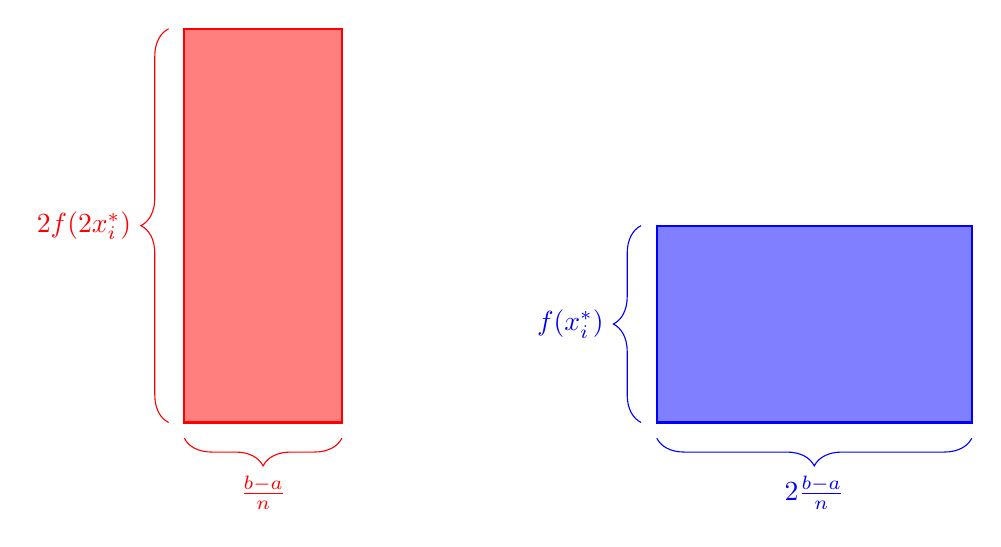
\begin{tikzpicture}
\color{red}
\draw[thick, fill=red, fill opacity=0.5] (0,0) rectangle (2,5);
\draw[decorate, decoration={brace, amplitude=10pt}] (2,-.2)--(0,-.2) node[midway, below, yshift=-10pt]{$\frac{b-a}{n}$};
\draw[decorate, decoration={brace, amplitude=10pt}] (-.2,0)--(-.2,5) node[midway, left, xshift=-10pt]{$2f(2x_i^*)$};
\color{blue}
\draw[thick, fill=blue, fill opacity=0.5] (6,0) rectangle (10,2.5);
\draw[decorate, decoration={brace, amplitude=10pt}] (10,-.2)--(6,-.2) node[midway, below, yshift=-10pt]{$2\frac{b-a}{n}$};
\draw[decorate, decoration={brace, amplitude=10pt}] (5.8,0)--(5.8,2.5) node[midway, left, xshift=-10pt]{$f(x_i^*)$};
\end{tikzpicture}
\end{center}

In the integral on the left, the variable is red $\textcolor{red}{x}$ and
in the integral on the right, the variable is blue $\textcolor{blue}{x}$.
Red $\textcolor{red}{x}$ and blue $\textcolor{blue}{x}$ are not the same. In fact $2\textcolor{red}{x_i^*}=\textcolor{blue}{x_i^*}$.
(Not every substitution corresponds to such a simple picture.)
\end{solution}

%%%%%%%%%%%%%%%%%%%
